\documentclass[a4paper]{article}
\usepackage[UTF8]{ctex}
\usepackage{geometry}
\usepackage{graphicx}
\usepackage{url}
\usepackage{multirow}
\usepackage{array}
\usepackage{booktabs}
\usepackage{url}
\usepackage{enumitem}
\usepackage{graphicx}
\usepackage{float}
\usepackage{amssymb}
\usepackage{amsmath}
\usepackage{subfig}
\usepackage{longtable}
\usepackage{pifont}
\usepackage{color}

\allowdisplaybreaks

\geometry{a4paper, scale=0.78}

\usepackage{tikz}
\newcommand*{\circled}[1]{\lower.7ex\hbox{\tikz\draw (0pt, 0pt)%
    circle (.5em) node {\makebox[1em][c]{\small #1}};}}

% \begin{figure}[H]
%     \centering
%     \includegraphics[width=.55\textwidth]{E.png}
%     \caption{矩阵与列向量的乘法}
%     \label{fig:my_label_1}
% \end{figure}

% \left\{
% \begin{array}{ll}
%       x+2x+z=2 & \\
%       3x+8y+z=12 & \\
%       4y+z=2
% \end{array}
% \right.

% \begin{enumerate}[itemindent = 1em, itemsep = 0.4pt, parsep=0.5pt, topsep = 0.5pt]

% \end{enumerate}

%\stackrel{a}{\longrightarrow}

%\underbrace{}_{} %下括号

%\tableofcontents %目录,并且目录页不记录页码
% \tableofcontents
% \newpage
% \setcounter{page}{1} %new page
% \clearpage

\title{Reinforcement Learning Markov Decision Process}
\author{Chen Gong}
\date{18 July 2020}
\begin{document}
%\pagestyle{empty}

\maketitle
\tableofcontents
\newpage
\setcounter{page}{1} %new page
%\pagestyle{fancy}
\section{Background}
Reinforcement Learning是一个比较成熟的学科,有着比较扎实的理论基础,同时也是我觉得深度学习中比较难的一个分支。强化学习主要是围绕马尔可夫决策过程(Markov Decision Process,MDP)来进行的。强化学习不同的流派使用的符号是不一样的,而我们这里和强化学习经典之作Sutton的“An introduction to reinforcement learning”中保持一致。那么,首先我们引出一下什么是MDP,

Random Variable:随机变量是整个概率论的基础,也是机器学习的基础。随机变量是用于某一随机变量发生的可能性。

Stochastic Process:举个小例子,就是股票的价格,令$t$时刻股价为$s_t$。股票的价格每个时刻都是不同的,价格都是服从一个分布的。而之前时刻股票的价格肯定都是对此时的价格都有影响。而$s_t,s_{t+1},s_{t+2},\cdots$关系非常的复杂。而$\{s_t\}_{t=1}^\infty$则为一个随机过程。

Markov Chain/Process:就是具有马尔可夫性质的随机过程。而Markov Property用公式表达为:$P(s_{t+1}|s_{t},s_{t-1},\cdots) = P(s_{t+1}|s_t)$。通俗的语言表达为,当前时刻的状态仅仅和上一个时刻的状态有关。这样可以简化计算,并具有一定的合理性。

State Space Model:包括哪些呢?有HMM,Kalman Filter,Particle Filter。状态空间模型,则为马尔可夫假设+观测独立假设。之所以有观测独立假设,是因为此模型中引入了隐变量。而某时刻观测变量只和此时刻隐变量之间有关系。

Markov Reward Process:此模型为Markov Chain+Reward。在两个状态之间发生转移的时候,会得到一个奖励。

Markov Decision Process:即为Markov Chain+Reward+Action。这里是怎么回事呢?两个相邻状态之间的转移受到action的影响,而且转移完成之后会得到一个reward,如下图所示。
\begin{figure}[H]
    \centering
    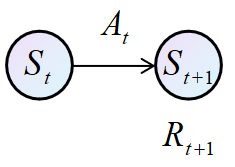
\includegraphics[width=.15\textwidth]{微信图片_20200719002902.png}
    \caption{MDP简要示意图}
    \label{fig:my_label_1}
\end{figure}
实际上MDP可以由一个四元组来表示$\langle \mathcal{S},\mathcal{A},\mathcal{P},\mathcal{R} \rangle$。其中$\mathcal{S}$表示的是状态集合,$\mathcal{A}$表示的是动作集合,$\forall s\in \mathcal{S}, A(s)\to a_t$;而$\mathcal{P}$是概率转移矩阵,表达两个状态之间转移的概率。$\mathcal{R}$为两个状态发生转移后得到的奖励。

\section{动态特征}
\subsection{完整的马尔可夫决策过程描述}
一个完整的MDP可以如下所示:
\begin{figure}[H]
    \centering
    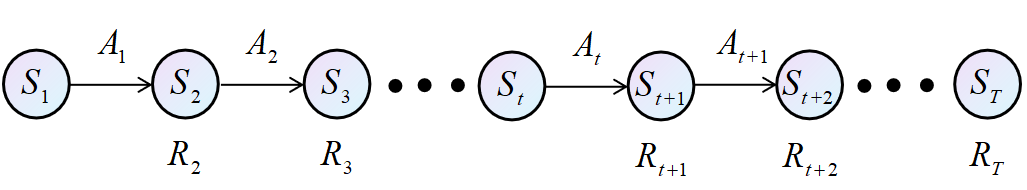
\includegraphics[width=.80\textwidth]{微信图片_20200719161809.png}
    \caption{MDP完整结构图}
    \label{fig:my_label_1}
\end{figure}
MDP在每个状态下,可以由个体从可能的行动空间$\mathcal{A}$ 中选择一个行动$a_t$,紧接着的状态转移概率随着所选择行动的不同而不同。另外,我们再加入即时奖励,就可以得到MDP的动态特征。
\begin{equation}
    P(s',r|s,a) = Pr\{ S_{t+1}=s',R_{t+1}=r|S_t=s,A_t=a \}
\end{equation}
我们注意到,马可夫性使得我们可以仅仅利用当前状态来估计接下来的收益,即仅仅使用当前状态来估计的策略并不比使用所有历史的策略差。可以说马可夫性带给我们了极大的计算上的便利,我们不用每一步都去处理所有的历史步骤,而是只需要面对当前的状态来进行处理。同时注意到,可能有些信息并没有被完整的包含到模型的状态信号$S_t$中,这使得模型并不满足马可夫性。不过我们一般还是认为它们是近似地满足马可夫性的,因此仅仅使用当前状态的信息来做出对于未来收益的预测和行动的选择并不是很差的策略。同时,如果选取不仅仅是当前时刻的状态状态,而是之前的多个时刻的状态叠加在一起作为当前状态,一般可以增强马可夫性。

而实际上$R_{t+1}$是随机变量,就算$S_t,A_t$一样,也有可能会有细微的差别。所以,状态转移函数被写为:
\begin{equation}
    P(s'|s,a) = \sum_{r\in \mathbb{R}} P(s',r|s,a)
\end{equation}
而其中奖励函数可以定义为:
\begin{equation}R\left(s^{\prime}, s, a\right)=\mathbb{E}\left[R_{t+1} \mid S_{t}=s, A_{t}=a, S_{t+1}=s^{\prime}\right]=\frac{\sum_{r \in \mathbb{R}} r p\left(s^{\prime}, r \mid s, a\right)}{p\left(s^{\prime} \mid s, a\right)}\end{equation}
类似地,我们还可以得到在状态$S_t$下,采取动作$a_t$将会得到的奖励为:
\begin{equation}R(s, a)=\mathbb{E}\left[R_{t+1} \mid S_{t}=s, A_{t}=a\right]=\sum_{r \in \mathbb{R}} r \sum_{s^{\prime} \in \mathcal{S}} p\left(s^{\prime}, r \mid s, a\right)\end{equation}

\subsection{强化学习最终目的}
强化学习的核心是决策,而MDP想要找到最优策略。那么什么是Policy呢?Policy的主要是为了得到$a_t$。Policy用$\pi$表示,1. 确定性策略,表示输出的动作是确定的$a=\pi(s)$;2. 随机性策略,$\pi(a|s) = Pr(A_t=a|S_t=s)$,此时输出的是动作$a$的概率分布。那么知道策略是什么以后,下一个问题则是,什么样的策略才是好的呢?

一般来说,Reward越高,即为获得了回报越高,策略越好。
\begin{equation}
    \begin{aligned}
    G_t = & R_{t+1} + \gamma R_{t+2} + \gamma^2 R_{t+2} + \cdots + \gamma^{r-T-1} R_T \\
    = & \sum_{i=0}^\infty \gamma^i R_{t+i+1}
    \end{aligned}
\end{equation}
其中,$R_{t+1}=R\left(S_{t+1}, S_{t}, A_{t}\right)$,$\gamma \in [0,1]$表示为衰减因子。
\begin{figure}[H]
    \centering
    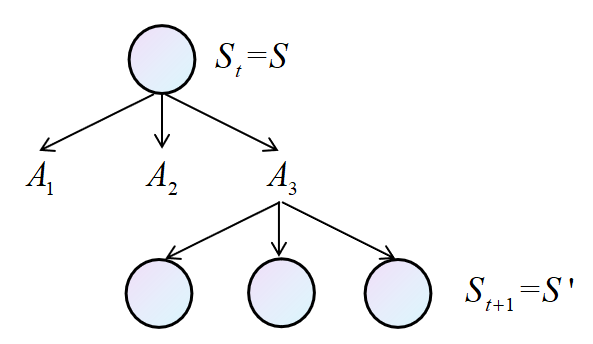
\includegraphics[width=.50\textwidth]{微信图片_20200720005916.png}
    \caption{MDP转移示例}
    \label{fig:my_label_1}
\end{figure}
实际上一个转移就是其中一条线,此图例中可以看到一共有9种转移可能,可以记为$G_t^{1},G_t^{2},\cdots,G_t^{9}$。并不是一个单独的$G_t$。所以,我们就可以用这个9个可能的平均值来表示最终的衡量标准。而实际中由于可能性很多,通常通过蒙特卡罗采样来求平均值得到最终的函数值,也就是价值函数:
\begin{equation}
    V^\pi(s) = \mathbb{E}_{\pi}[G_t|S_t=s]
\end{equation}

\section{价值函数(Value Function)}
确定性策略可以看成是一种特殊的随机性策略。在前文中已经引出了价值函数$V^\pi(s)$的概念,实际上$V^\pi(s)$是一个列向量,列向量的维度就为$|s|\times 1$,有多少个状态就有多少个$V^\pi(s)$。下面将给出价值函数和状态价值函数的定义,
\begin{equation}\begin{array}{l}
V^{\pi}(s)=\mathbb{E}_{\pi}\left[G_{0} \mid S_{0}=s\right]=\mathbb{E}\left[\sum_{t=0}^{\infty} \gamma^{t} R_{t+1} \mid S_{0}=s\right] \\
Q^{\pi}(s, a)=\mathbb{E}_{\pi}\left[G_{0} \mid S_{0}=s, A_{0}=a\right]=\mathbb{E}\left[\sum_{t=0}^{\infty} \gamma^{t} R_{t+1} \mid S_{0}=s, A_{0}=a\right]
\end{array}\end{equation}
其中函数$V^\pi(s)$表示的是当到达某个状态$s$之后,如果接下来一直按着策略$\pi$来行动,能够获得的期望收益;函数$Q^\pi(s,a)$表示的是当达到某个状态$s$之后,如果采取行动$a$,接下来再按照策略$\pi$来行动,能获得的期望收益。

这里有一个区别需要特别说明一下,$\pi$实际上就是一个状态到动作的映射,$\pi:s \to a$。在$V^\pi(s)$中$\pi$对$s$是有约束的,因为,在这个函数中$a$的选择是和$\pi$有关的;而在$Q^{\pi}(s, a)$就不是这样了,$\pi$对$s$是没有约束的,$s,a$在此函数中仅仅是两个自变量,彼此之间并没有关系,不是由$\pi:s \to a$的关系得出的。

而$V^\pi(s)$和$Q^{\pi}(s, a)$之间的关系可以写为:
\begin{equation}
    \begin{aligned}
    V^\pi(s) = & Q^{\pi}(s, a) = \pi(a_1|s)Q^\pi(s,a_1) + \pi(a_2|s)Q^\pi(s,a_2) + \pi(a_3|s)Q^\pi(s,a_3) + \cdots \\
    = & \sum_{a\in\mathcal{A}(s)} \pi(a|s)\cdot Q^\pi(s,a)
    \end{aligned}
\end{equation}
我们可以看到$V^\pi(s) = \sum_{a\in\mathcal{A}(s)} \pi(a|s)\cdot Q^\pi(s,a)$实际上是一个加权平均值。我们已经知道了它们两之间的这层关系,那么还有别的关系吗?显而易见的是,
\begin{equation}
    V^\pi(s) \leq \max_a Q^\pi(s,a)
\end{equation}
因为$V^\pi(s)$是$Q^\pi(s,a)$的加权平均值。

$P(s',r|s,a)$中$s',r$都是具有随机性的。而递归地展开(7)中的两个公式即可得到相应的两个Bellman方程(Bellman equation),对于$V^\pi(s)$的式子,有:
\begin{equation}\begin{aligned}
V^{\pi}(s) &=\mathbb{E}_{\pi}\left[\sum_{t=0}^{\infty} \gamma^{t} R_{t+1} \mid S_{0}=s\right] \\
&=\mathbb{E}_{\pi}\left[R_{t+1}+\gamma \sum_{k=0}^{\infty} \gamma^{t} R_{t+2} \mid S_{1}=s\right] \\
&=\sum_{a} \pi(a \mid s) \sum_{s^{\prime}} \sum_{r} p\left(s^{\prime}, r \mid s, a\right)\left[r+\gamma \mathbb{E}_{\pi}\left[\sum_{t=0}^{\infty} \gamma^{t} R_{t+2} \mid S_{1}=s^{\prime}\right]\right] \\
&=\sum_{a} \pi(a \mid s) \sum_{s^{\prime}, r} p\left(s^{\prime}, r \mid s, a\right)\left[r+\gamma V^{\pi}\left(s^{\prime}\right)\right] \\
& \forall s \in \mathcal{S}
\end{aligned}\end{equation}
同理,把$\sum_{a} \pi(a \mid s)$去掉就得到了$Q^\pi(s,a)$的Bellman方程:
\begin{equation}
\begin{aligned}
    Q^\pi(s,a) = & \sum_{s^{\prime}, r} p\left(s^{\prime}, r \mid s, a\right)\left[r+\gamma V^{\pi}\left(s^{\prime}\right)\right] \\
    = &\sum_{s^{\prime}, r} p\left(s^{\prime}, r \mid s, a\right)\left[r+\gamma \sum_{a'\in\mathcal{A}(s')} \pi(a'|s')\cdot Q^\pi(s',a') \right] \\
\end{aligned}
\end{equation}
这就是Bellman Expectation Function。

\section{Bellman最优方程}
上一小节中,主要介绍了价值函数和状态价值函数之间的关系,并推导出了两个Bellman方程。注意,强化学习的目的就是找到最优的$\pi$,算法中可以优化的也只有$\pi$。$V^\pi(s)$是我们的优化目标,为了找到这个最优的$V^\ast(s)$才引入了最优价值函数的概念。同时,我们把可以使得价值函数达到最大的那个$V^\pi(s)$称之为最优价值函数。定义如下所示:
\begin{equation}\left\{\begin{array}{l}
V^{*}(s) \stackrel{\Delta}{=} \max_\pi V^{\pi}(s) \\
Q^{*}(s, a) \stackrel{\Delta}{=} \max_\pi Q^{\pi}(s, a)
\end{array}\right.\end{equation}
首先能够使得$\pi$到达最优的策略可能有多个,为了表达方便,就假设只有一个,那么记,
\begin{equation}
    \pi^\ast = \underset{\pi}{\arg\max} V^\pi(s) = \underset{\pi}{\arg\max} Q^\pi(s,a)
\end{equation}
那么,很显然可以得到:
\begin{equation}
    V^\ast(s) = \max_\pi V^\pi(s) = V^{\pi^\ast}(s)
\end{equation}
\begin{equation}
    Q^\ast(s,a) = \max_\pi Q^\pi(s,a) = Q^{\pi^\ast}(s,a)
\end{equation}
同时需要注意的是,$ V^\ast(s)$和$V^{\pi^\ast}(s)$看上去是一模一样的,实际上它们分别属于不同的意义。最优价值函数$V^\ast(s)$隐去了策略和$\pi$没有关系,它仅仅是一个函数。而$V^{\pi^\ast}(s)$是一个普通的价值函数,它表示的是有最优的$\pi$得出的价值函数。

那么,我们下一步的想法就是可不可以如同公式(11)一样,构建$V^\ast(s)$和$V^\ast(s’)$,$Q^\ast(s,a)$和$Q^\ast(s',a')$来方便我们进行求解。

首先,我们要知道$V^{\pi^\ast}(s)$和$Q^{\pi^\ast}(s,a)$之间有什么样的关系。由于,前面的小节中讲到了$V$函数是$Q$函数的一个加权平均,那么显然可以得到:
\begin{equation}
    V^{\pi^\ast}(s) \leq \max_a Q^{\pi^\ast}(s,a)
\end{equation}
由于$\pi^\ast$就是一个最优的策略,所以直觉上我们会觉得,应该是
\begin{equation}
    V^{\pi^\ast}(s) = \max_a Q^{\pi^\ast}(s,a)
\end{equation}
那么有没有可能会是小于呢?如果$V^{\pi^\ast}(s) < \max_a Q^{\pi^\ast}(s,a)$那意味着平均值小于最大值,则说明$\pi^\ast$肯定还有提高的空间,则不是最优策略。必然存在一个$\pi_{\text{new}} \neq \pi^\ast$使得$\pi_{\text{new}} =\max$,这显然与$\pi^\ast$是最优策略的前提是矛盾的。当然这些只是我们直觉上推断,有的同学会问,这个$\pi_{\text{new}}$到底是长什么样呢?下面我们来构造证明一下:

假设,$V^{\pi^\ast}(s) < \max_a Q^{\pi^\ast}(s,a)$,可以构造$\pi_{\text{new}}$,我们假设它是一个确定性策略,
\begin{equation}
    \pi_{\text{new}} =
    \left\{
    \begin{array}{ll}
        \pi_{\text{new}}(s) = \max_a Q^{\pi^\ast}(s,a) & \forall s\in \mathcal{S}  \\
        \pi_{\text{new}}(\bar{s}) = \pi^\ast(\bar{s}) & \forall \bar{s} = \mathcal{S} - s
    \end{array}
    \right.
\end{equation}
也就是出了$s$状态的动作等于$\max_a Q^{\pi^\ast}(s,a)$,其他的动作都不变。那么就有
\begin{equation}
    V^{\pi_{\text{new}}}(s) = \max_a Q^{\pi^\ast}(s,a) > V^{\pi^\ast}(s)
\end{equation}
显然$\pi_{\text{new}}$优于$\pi^\ast$,所以与我们的假设冲突,所以,必然有$V^{\pi^\ast}(s) = \max_a Q^{\pi^\ast}(s,a)$。而我们看到这个式子实际上就是公式(8)把那个加权平均给拿掉了。其他的公式(10,11)可不可以做类似变换,那必然是不行的,因为公式(8)中的动作是人为可以选择的,而(10,11)中包含$s$的变化,这是环境给出的,不能人为控制。那么,同样我们可以建立最优策略中$s,s'$之间的关系,
\begin{equation}\begin{aligned}
V^{*}(s) &=\max _{a \in \mathcal{A}(s)} \sum_{s^{\prime}, r} p\left(s^{\prime}, r \mid s, a\right)\left[r+\gamma V^{*}\left(s^{\prime}\right)\right] \\
& = \max _{a \in \mathcal{A}(s)} \sum_{s^{\prime}, r} p\left(s^{\prime}, r \mid s, a\right)\left[r+\gamma \max_a Q^\ast(s,a)\right] \\
Q^{*}(s, a) &=\sum_{s^{\prime}, r} p\left(s^{\prime}, r \mid s, a\right)\left[r+\gamma \max _{a^{\prime}} Q^{*}\left(s^{\prime}, a^{\prime}\right)\right]
\end{aligned}\end{equation}
这就是Bellman Optimality Equation。最后再提一点,在很多参考文献中,为了简便表示通常使用期望的方式来表达价值函数。
\begin{equation}
    V^\pi(s) = \mathbb{E}^\pi\left[R_{t+1} + \gamma V^\pi(s_{t+1})|s_t=s\right]
\end{equation}


\section{贝尔曼算子}
此小节是对老师的内容做的一个小小的补充。简单讲解一下贝尔曼方程的收敛性,需要用到压缩映射定理。

在前一节中我们定义了两种价值函数,如果能够求得在某策略下的价值函数,我们就可以对该策略的好坏进行评估;如果能够求得最优情形下的价值函数,我们就可以自然得出最优策略。但我们还不知道要如何计算得到相应的价值函数数值,我们这里引入的Bellman算子及其相关的性质,可以为相关算法的收敛性提供一些保证。

考虑有限的状态空间$\mathcal{S} = [n]$,和定义在状态空间上的实值函数$V^\pi$。定义贝尔曼算子$\mathcal{T}:\mathbb{R}^n \to\mathbb{R}^n$。
\begin{equation}(\mathcal{T} V)_{i}=\max _{a \in \mathcal{A}(i)} \sum_{j \in[n]} P(j \mid i, a)\left(R(j, i, a)+\gamma V_{j}\right)\end{equation}

其中下标都表示向量的某个元素。对于一个策略$\pi$还可以定义Bellman算子$\mathcal{T}^\pi:\mathbb{R}^n \to\mathbb{R}^n$,
\begin{equation}\left(\mathcal{T}_{\pi} V\right)_{i}=\sum_{j \in[n]} P(j \mid i, \pi)\left(R(j, i, \pi)+\gamma V_{j}\right)\end{equation}
对于确定性策略来说$\pi$的输出就是一个动作,对于随机策略则还需要对整体取期望。

\textbf{定理3.1(压缩映射定理,Banach不动点定理)}设函在区间$[a,b]$上定义$f([a,b])\subset (a,b)$,存在一个常数$\beta \in [0,1]$,使得对于一切$u,v \in [a,b]$,使得不等式成立$|f(u)-f(v)|\leq \beta(u-v)$,则将称为$f$上的一个压缩映射,则称常数$\beta \in [0,1]$为压缩常数。记为,并且用无穷范数来定义算子之间的距离。

将贝尔曼方程记为$$\mathcal{T}(u)=r_{t+1}+\eta P(\pi) u$$,并且用无穷范数来定义算子之间的距离。
\begin{equation}
    \begin{aligned}
d\left(|\mathcal{T}(u) - \mathcal{T}(v)\right) = & \left\|r_{t+1}+\gamma P(\pi) u - r_{t+1} - \gamma P(\pi) v \right\|_\infty \\
= & \left\|\gamma P(\pi) u - \gamma P(\pi) v \right\|_\infty \\
= & \left\|\gamma P(\pi) ( u - v ) \right\|_\infty \\ 
\leq &  \left\|\gamma P(\pi) \left\| u - v \right\|_\infty \right\|_\infty \\
\leq & \gamma \left\| u - v \right\|_\infty = \gamma d(u,v)
\end{aligned}
\end{equation}
所以,根据上述推导可以得出,1.贝尔曼方程可以唯一收敛于$V^\pi=V^{\pi^\ast}$,即为$\lim _{k \rightarrow \infty} \mathcal{T}^{k} V=V^{*}$,其中$k$为迭代次数;2. 算法以的线性速率收敛。那么通过压缩映射定理,可以推出值迭代算法的收敛性。这样就差不多可以了,很多新的算法中都是定义一个新的贝尔曼算子,然后通过压缩映射定理来证明其收敛性,最后用实验来进行说明。

\section{小结}
本章节主要是对强化学习的一个入门,介绍了强化学习的一些基本概念,从马尔可夫决策过程来引出强化学习,而强化学习的核心就是求一个策略$\pi:s\to a$,来满足决策的要求。然后介绍了如何评判一个马尔可夫决策过程的优劣,从而引出了价值函数和状态动作函数,两个评判函数。然后建立了这两个评判函数相邻状态之间的关系,即为Bellman方程。为了进一步简便运算,加快收敛从而引出了Bellman Optimality Equation,并推导了最优方程中,价值函数和状态动作函数之间的关系。最后,介绍了压缩映射定理证明了贝尔曼方程的迭代可以收敛到唯一的最优解。下一章则是具体介绍如何求解最优价值函数了。













\end{document}